\chapter{Introduction}
\label{chap:intro}
A gentle reminder not to get this chapter perfect until the dissertation is nearing its completion\ldots

\section{A section}
\label{intro:sections}

Use this to break up your chapters into logical parts

\subsection{A sub-section}

Use this to break up your sections into smaller logical parts

\subsubsection{A sub-sub-section}

Use this one more sparingly... if you are finding yourself in nesting depth 4 you are probably overdoing it, or this section should have been its own chapter.

\paragraph{The last and fifth heading provided} is the paragraph command (ok there is subparagraph but seriously\ldots)

\section{Citations}
\label{intro:citations}

When it comes to referencing, if we want to assert a fact and then provide its reference use \verb!\parencite!. For example -- one should adapt feedback to learner personality \parencite{dennis2016adapting}.

Or if you want to talk about the research directly, use \verb!\textcite!: \textcite{dennis2016adapting} did a PhD in adapting feedback to learner personality. 

If you want to cite two sources at the same time, you can separate the keys with commas \parencite{dennis2016adapting,cle12}.

\textcite{dennisiui} blah. \textcite{ruta2018websight} was an awesome paper.

\section{Quotations}
\label{intro:quotations}
We have added the \verb|\bq[author]{authors words here}| blockquote macro to make block quotes simple.  Gnerally we discourage quoting large sections of text in favour of ciritique, summary and paraphrasing.

\bq[Obiwan Kenobi]{Remember, a Jedi can feel the paraphrase flowing through them.  Stretch out with your critical evaluation Luke.}

Old Obi-wan was also well known for saying \qq{use the force}. 

\section{Figures}
\label{intro:figures}

\begin{figure}
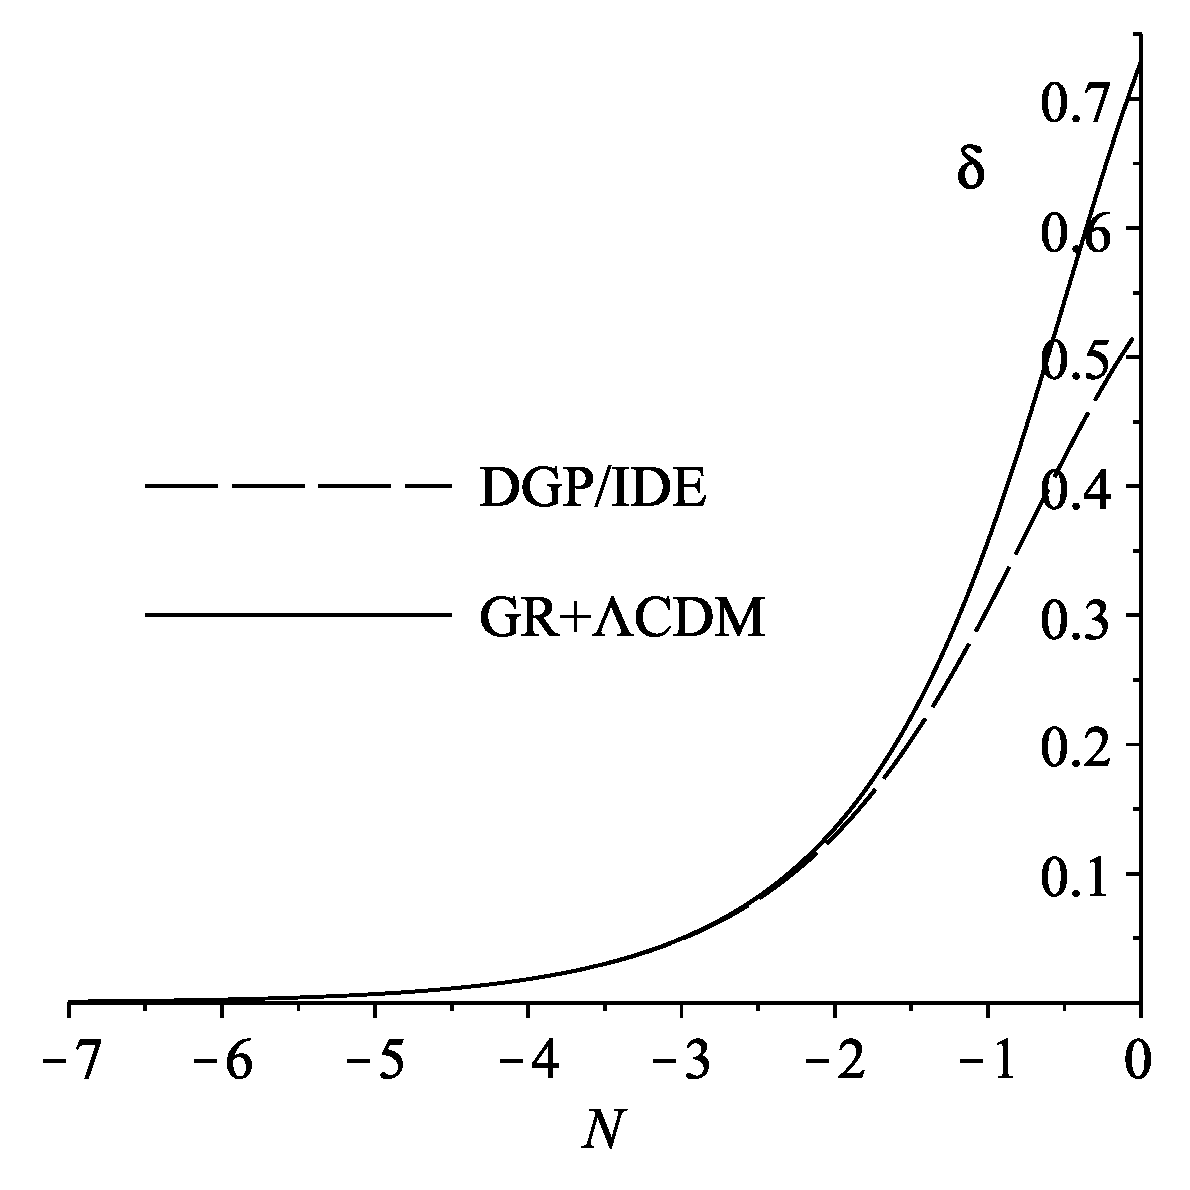
\includegraphics[width=0.49\columnwidth]{figures/dgpdeltas.eps}
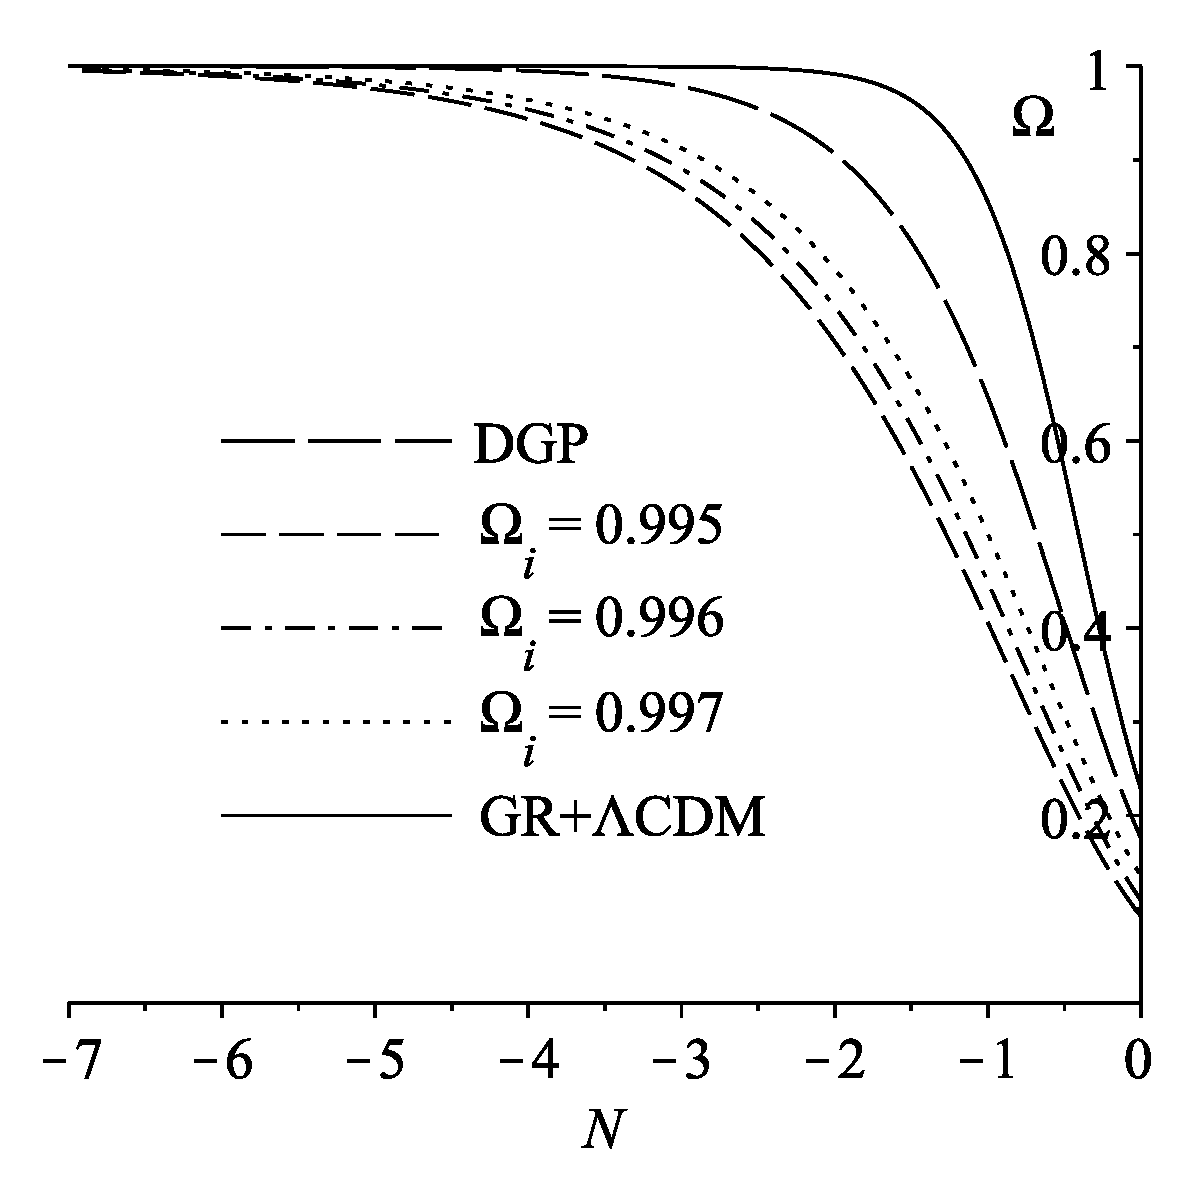
\includegraphics[width=0.49\columnwidth]{figures/dgpomegas.eps}
% For long captions include a short version for the List of Figures/Tables sections in square brackets as below.
\caption[Evolutions of $\delta$ and $\Omega$ for DGP]{Evolution of the density perturbation (left) and the density parameters (right) for the matched DGP/IDE models, each with a different $\Omega_i$,
and a GR+$\Lambda$CDM model.
\label{fig:matched}}
\end{figure}

Don't the graphs in \autoref{fig:matched} look scary? Don't worry, this is because I adapted this template from ICJS. Remember -- if you are including screenshots or other raster graphics (i.e. PNG, JPEG) you should ensure that they are at least 300dpi. This will take effort on your part -- most people's screens are at 72dpi.   

Vector is better (EPS or PDF) if you can manage it. If you are exporting graphs from Microsoft Excel for example, place the chart in its own sheet and print it to PDF. Then, using Acrobat or similar, crop the whitespace off the PDF. This is the most reliable way I have found to include vector graphics from Microsoft Office.

Remember, it's \LaTeX's job to position the images for you.  You put them in the document approximately in the right place and let \LaTeX  do all the work. 





% To include math symbols in things with hyperlinks you need to specify an alternative plain text version for the bookmark using \texorpdfstring as below:
\section{A section with math symbols, eg. \texorpdfstring{$\Lambda$}{Lambda}CDM}
test test test test test test test test test test test test test test test test test test test test
test test test test test test test test test test test test test test test test test test test test
test test test test test test test test test test test test test test test test test test test test
test test test test test test test test test test test test test test test test test test test test
test test test test test test test test test test test test test test test test test test test test
test test test test test test test test test test test test test test test test test test test test
test test test test test test test test test test test test test test test test test test test test
test test test test test test test test test test test test test test test test test test test test

\section{Cross References}

This chapter has introduced several topics, and this section summarises these and introduces cross references to each, before looking forward to other parts of the document.

In opening, \textit{Sections} were introduced \see{intro:sections}.  Then key aspects of \nameref{intro:citations} \see{intro:citations} and \nameref{intro:quotations} \see{intro:quotations} were summarised, before the use of \nameref{intro:figures} \see{intro:figures} was clealy demonstrated.  

Each of the cross references in the above paragraph uses (i.e. refers to) a label.  Labels are defined using \verb|\label{example:name}|.  When naming a label, we often add the name of the chapter (or an abbreviation of it) which reduces the chance of names clashing, or choosing a lookalike by mistake.  If you look at the source of this page you'll see that the cross referenced labels are all defined as \verb|\label{intro:name}|, where \textit{name} is different for each label.

It's these labels we're referring to when we make cross references.  In the next paragraph we used \verb|\nameref{lr}| to insert the name of the literature review chapter (so if that chapter name changes, the reference will update too).  We then used \verb|\seenamed{lr}| to add the longer text reference that can be followed if/when the work is printed out.

Looking forward, the \nameref{lr} chapter is a great example of how different files can be used for chapters \seenamed{lr}.
